% This is ''sig-alternate.tex'' V2.0 May 2012
% This file should be compiled with V2.5 of '\'sig-alternate.cls'' May 2012
%
% This example file demonstrates the use of the \'sig-alternate.cls'
% V2.5 LaTeX2e document class file. It is for those submitting
% articles to ACM Conference Proceedings WHO DO NOT WISH TO
% STRICTLY ADHERE TO THE SIGS (PUBS-BOARD-ENDORSED) STYLE.
% The \'sig-alternate.cls' file will produce a similar-looking,
% albeit, 'tighter' paper resulting in, invariably, fewer pages.

\documentclass{sig-alternate}
\usepackage{paralist}
\usepackage{url}

%
\def\sharedaffiliation{%
\end{tabular}
\begin{tabular}{c}}
%
\begin{document}
%
% --- Author Metadata here ---
\conferenceinfo{WIPSCE}{2015 London, UK}
\CopyrightYear{2015} % Allows default copyright year (20XX) to be over-ridden - IF NEED BE.
%\crdata{0-12345-67-8/90/01}  % Allows default copyright data (0-89791-88-6/97/05) to be over-ridden - IF NEED BE.
% --- End of Author Metadata ---

% working title!
\title{Using Interface Design to Develop\\Computational Thinking Skills}
%Interface Design and Its Role in Computational Thinking
%Thinking About Design, Thinking About Computing?
%The Interface Between Design and Computational Thinking?


\numberofauthors{2}
\author{
% 1st. author
\alignauthor
Ana C. Calderon\\
\affaddr{Department of Computing}\\
\affaddr{Cardiff Metropolitan University, UK}\\
\affaddr{acalderon@cardiffmet.ac.uk}
% 2nd. author
\alignauthor
Tom Crick\\
\affaddr{Department of Computing}\\
\affaddr{Cardiff Metropolitan University, UK}\\
\affaddr{tcrick@cardiffmet.ac.uk}\\
}

\maketitle

\begin{abstract}
Human-computer interaction is a long established sub-discipline of
computer science. While there has been significant focus on the
importance of developing computational thinking skills, there appears
to be a gap in the literature in using HCI principles, analysis and
design as a framework for doing so. We present the first step to
identify methodologies for systematically introducing HCI to pupils
from an early age, presenting a commentary for their prospective
future application, comparing to similar approach as other
foundational aspects of computer science in developing computational
thinking skills that have been considered for the past decade.
\end{abstract}

% A category with the (minimum) three required fields
\category{K.3.2}{Computers \& Education}{Computer and Information Science Education}[Computer Science Education]
\keywords{Computer Science Education; Computational Thinking; HCI; Design; Interaction}

\section{Introduction}

Computational thinking is increasingly valued for its significance in
the teaching of foundations of computer science as well as its ability
to aid broader problem-solving skills across a range of
subjects~\cite{brown-et-al-sigcse2012,brown-et-al-toce2014}. HCI is a
well established research and application area in computer science,
but it is also a multi-disciplinary domain which, we argue, has a
number of important links to computational thinking. Interactivity and
design has been a somewhat undervalued theme during the growth of
computational thinking as a high-value skill, with an associated gap
in the literature. Some proof-of-concept solution methodologies are
detailed, targeted at particular aspects of HCI, presented in the form
of sessions accessible to children of primary school age.

\section{Suggested sessions}

We now give methodologies, in the form of activity-based learning
sessions, to teach elements crucial to HCI to secondary school
students. These are ideas are influence by
Norman~\cite{norman2002design}, Rogers~\cite{rogers2011interaction}
and Shneiderman~\cite{shneiderman1986designing}.

\subsection{Session A}

The first session we describe is intended to cover negative transfer
as well as the principle of affordance, and we break down the
explanation not by the flow of the session, but by the intended
learning outcome, this is intended to facilitate also the explanation
of the effects making the presentation accessible outside the HCI
community. The session was devised with the use of a ``doll house''
specifically designed in a self-contradictory manner. The students are
given clues to navigate around the house and their goal is to find a
pebble. To find the hidden pebble, the students must follow
instructions and activities specified in the cards. This follows
similar patterns as a popular game show, and the reason is to help the
students view this as a fun activity rather than a typical learning
session (via traditional classroom environments).

\subsubsection*{Principle of affordance}

Affordances are the product of agents and their environment
\cite{gibson1977theory}, gien any agent-environment combination a
affordance may or may not exist. If one does the agent needs to be
aware of it, however for most HCI researchers when affordance is
mentioned it is typically assumed that the agent is aware of it, calls
this a perceived affordance \cite{norman1999affordance}.

The very first instruction given to students is to simply enter the
house, the entrance consists of a front door, porch, both doors have a
door knob, the first door must be pushed whereas the second door needs
to be pulled. Students are likely to try to turn the knob the first
time and push the second. At this stage in the session, an explanation
is due, on how past experiences can affect learning of new tasks. In
addition most students are likely to attempt to turn the knob, which
makes it an excellent point to teach students about the principle of
affordance.


\subsubsection*{Explaining transfer effects applied to design methods
  in HCI}

Negative transfer\cite{Lunchin, Pan2010, Woltz} is a term in
behavioural psychology to describe how new task learning can be
negatively affected by knowledge of similar or related tasks.  This
has consequences to design of interactive designs
\cite{waern1993varieties} For example,\cite{Besnard2005105} uses a
simulated experiment (based on real industrial work environments) to
support a hypothesis of how interface changes are less likely to cause
accidents when it limits changes to former interaction patterns.

Amongst the instructions, pupils are asked to fill up a watering can
in the kitchen, water the plants, return to the house and clean the
same watering can in the downstairs guest bathroom. The first tap used
must be turned clockwise in order to let out water, conversely the
second tap must be turned anti-clockwise for the same goal to be
achieved. This is the second intentional opportunity during the
activity, in which teachers can explain transfer effects and start a
discussion bout its importance to design.

\subsection{Session B}

The second session is based on a similar activity as published in
\cite{fellows2005} where students are given cooking ingredients lists
to transform into symbols.

\subsubsection*{Design for recognition}
 
As the above section demonstrate, learning how to achieve certain
tasks will have consequences to learning new tasks. As humans we are
constantly learning new skills and it is thus essential to design
intuitive interactive devises. The following two sessions are aimed at
highlighting the importance of designing to minimise the amount of
learning required.

For this, pupils are placed into two groups, the first group is given
three lists: ingredients, portions and instructions. They must find a
way to abstract away from the textual information and draw icons and
symbols that will aid the second group of pupils put together a
recipe. The list is small, ``chocolate, milk, butter'' and the portions
are simple ``a little'', ``a lot'', ``a big piece'', ``a medium piece'', the
instructions are also simple ``start mixing'', ``stop mixing'', ``start
pouring'', etc. The students should enjoy themselves as they try to
discover whether how close to the original recipe the second group's
recipe is. After the session is complete the teacher should emphasise
their learning of difficult but important it is to design interfaces
with icons that are meaningful. Examples of solutions to text
abstraction can be found in \ref{fig1} (representing small, medium
and large piece).


\begin{figure}
  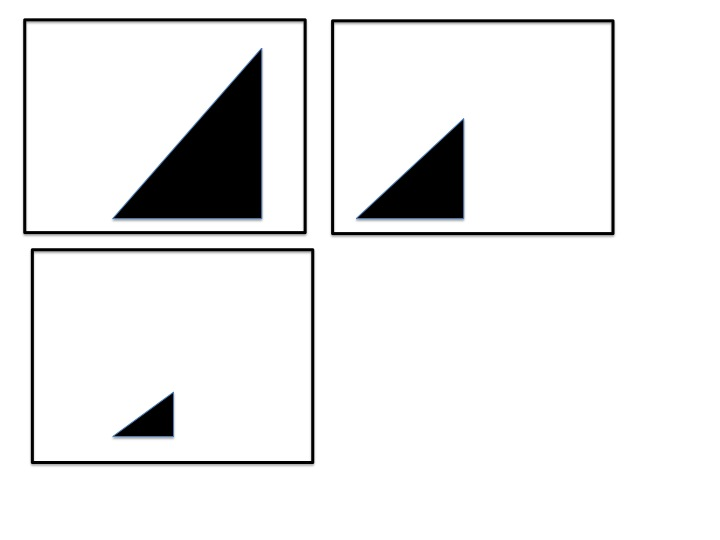
\includegraphics[width=\columnwidth]{images/portions.jpg}
  \caption{Example of representing portions via text.}\label{fig1}
\end{figure}

\subsubsection*{Iterative Design}

Iterative design: After determining the users, tasks, and empirical
measurements to include, perform the following iterative design steps:

\begin{itemize}
\item Design the user interface; 
\item Test;
\item Analyse results;
\item Repeat;
\item Repeat the iterative design process until a sensible, user-friendly interface is
created.
\end{itemize}

In addition, this session can be structured to teach other
design-relevant methodologies to children, namely iterative
design. This is achieved by allowing the pupils second and third
attempts at their representation of the text given to them (we expect
more than three attempts would be frustrating for the pupil, and three
are enough to illustrate the principle of iteration in design). The
pupils must be told that the iteration is intended to improve the
design and should be repeated until a good and sensible set of symbols
is achieved (as would happen with an interface with programmers). This
should be followed by a short formative session on iterative design,
highlighting the main concepts in a language accessible to the
particular age group, for instance:

\begin{enumerate}
\item What is the target audience of your interactive software? What
  is the goal of your software? What empirical testing can be done to
  check for accuracy in achieving the tasks post creation of your
  interface?
\item Design your interface 
\item Test your interface
\item Interpret results
\item Iterate (repeat)
\item End when satisfied with resulting interface
\end{enumerate}

The sessions described are intended as examples of principles relevant
to HCI, this is the beginning of a list of potentially several
principles that are important to HCI, we mean for this sessions to be
seen as illustrative examples rather than containing a comprehensive
list of principles.


%%%
\section{Conclusions}

We have presented a methodology for introducing rigorous design
principles and theories relevant to human-computer interaction to
young children. This is exemplified with two sessions developed
encompassing computational thinking. We hypothesise that HCI can be
embedded as a valuable part of developing computational thinking
skills in young students, and that these will have a positive impact
more broadly across their future learning, not just for computer
science. Furthermore, we reiterate the wider societal benefits of
developing these broad computational skills, both as baseline digital
competencies to ensure a digitally engaged citizenry, as well as high
value skills for the economies of the future. Immediate future work
will consist of an implementation of the sessions with a cohort of
students to investigate their feasibility as part of a scheme of work
and how they progress over an academic period.

% bib
\bibliographystyle{abbrv}
\bibliography{wipsce2015}


% \section*{To Do}

% In no particular order...

% \begin{itemize}
% \item Add stuff here...
% \end{itemize}

% \subsection*{References to use}
% \begin{itemize}
% \item
% General CAS
% citations~\cite{crick+sentance:2011,brown-et-al-sigcse2012,brown-et-al-toce2014}.

% \item
% Teachers, CPD and
% NoE~\cite{sentance-et-al-wipsce2012,sentance-et-al:2013,sentance-et-al:2014}.

% \item
% Welsh Government reports/policy:
% \begin{itemize}
% \item
% ICT Review~\cite{welshictreview:2013}
% \item
% Graham Report on STEM~\cite{STEMreview:2014}
% \item
% Donaldson Report~\cite{Donaldson:2015}
% \item
% Furlong Report~\cite{Furlong:2015}
% \end{itemize}

% \item
% Misc Reports
% \begin{itemize}
% \item
% Nesta report~\cite{NESTA:2015}

% \end{itemize}
% \end{itemize}

\end{document}
